%% BioMed_Central_Tex_Template_v1.06
%%                                      %
%  bmc_article.tex            ver: 1.06 %
%                                       %

%%IMPORTANT: do not delete the first line of this template
%%It must be present to enable the BMC Submission system to 
%%recognise this template!!

%%%%%%%%%%%%%%%%%%%%%%%%%%%%%%%%%%%%%%%%%
%%                                     %%
%%  LaTeX template for BioMed Central  %%
%%     journal article submissions     %%
%%                                     %%
%%         <14 August 2007>            %%
%%                                     %%
%%                                     %%
%% Uses:                               %%
%% cite.sty, url.sty, bmc_article.cls  %%
%% ifthen.sty. multicol.sty		   %%
%%				      	   %%
%%                                     %%
%%%%%%%%%%%%%%%%%%%%%%%%%%%%%%%%%%%%%%%%%


%%%%%%%%%%%%%%%%%%%%%%%%%%%%%%%%%%%%%%%%%%%%%%%%%%%%%%%%%%%%%%%%%%%%%
%%                                                                 %%	
%% For instructions on how to fill out this Tex template           %%
%% document please refer to Readme.pdf and the instructions for    %%
%% authors page on the biomed central website                      %%
%% http://www.biomedcentral.com/info/authors/                      %%
%%                                                                 %%
%% Please do not use \input{...} to include other tex files.       %%
%% Submit your LaTeX manuscript as one .tex document.              %%
%%                                                                 %%
%% All additional figures and files should be attached             %%
%% separately and not embedded in the \TeX\ document itself.       %%
%%                                                                 %%
%% BioMed Central currently use the MikTex distribution of         %%
%% TeX for Windows) of TeX and LaTeX.  This is available from      %%
%% http://www.miktex.org                                           %%
%%                                                                 %%
%%%%%%%%%%%%%%%%%%%%%%%%%%%%%%%%%%%%%%%%%%%%%%%%%%%%%%%%%%%%%%%%%%%%%


\NeedsTeXFormat{LaTeX2e}[1995/12/01]
\documentclass[10pt]{bmc_article}    



% Load packages
\usepackage{graphicx}
\usepackage{cite} % Make references as [1-4], not [1,2,3,4]
\usepackage{url}  % Formatting web addresses  
\usepackage{ifthen}  % Conditional 
\usepackage{multicol}   %Columns
\usepackage[utf8]{inputenc} %unicode support
%\usepackage[applemac]{inputenc} %applemac support if unicode package fails
%\usepackage[latin1]{inputenc} %UNIX support if unicode package fails
\urlstyle{rm}
 
 
%%%%%%%%%%%%%%%%%%%%%%%%%%%%%%%%%%%%%%%%%%%%%%%%%	
%%                                             %%
%%  If you wish to display your graphics for   %%
%%  your own use using includegraphic or       %%
%%  includegraphics, then comment out the      %%
%%  following two lines of code.               %%   
%%  NB: These line *must* be included when     %%
%%  submitting to BMC.                         %% 
%%  All figure files must be submitted as      %%
%%  separate graphics through the BMC          %%
%%  submission process, not included in the    %% 
%%  submitted article.                         %% 
%%                                             %%
%%%%%%%%%%%%%%%%%%%%%%%%%%%%%%%%%%%%%%%%%%%%%%%%%                     


%\def\includegraphic{}
%\def\includegraphics{}



\setlength{\topmargin}{0.0cm}
\setlength{\textheight}{21.5cm}
\setlength{\oddsidemargin}{0cm} 
\setlength{\textwidth}{16.5cm}
\setlength{\columnsep}{0.6cm}

\newboolean{publ}

%%%%%%%%%%%%%%%%%%%%%%%%%%%%%%%%%%%%%%%%%%%%%%%%%%
%%                                              %%
%% You may change the following style settings  %%
%% Should you wish to format your article       %%
%% in a publication style for printing out and  %%
%% sharing with colleagues, but ensure that     %%
%% before submitting to BMC that the style is   %%
%% returned to the Review style setting.        %%
%%                                              %%
%%%%%%%%%%%%%%%%%%%%%%%%%%%%%%%%%%%%%%%%%%%%%%%%%%
 

%Review style settings
%\newenvironment{bmcformat}{\begin{raggedright}\baselineskip20pt\sloppy\setboolean{publ}{false}}{\end{raggedright}\baselineskip20pt\sloppy}

%Publication style settings
%\newenvironment{bmcformat}{\fussy\setboolean{publ}{true}}{\fussy}

%New style setting
\newenvironment{bmcformat}{\baselineskip20pt\sloppy\setboolean{publ}{false}}{\baselineskip20pt\sloppy}

% Begin ...
\begin{document}
\begin{bmcformat}


%%%%%%%%%%%%%%%%%%%%%%%%%%%%%%%%%%%%%%%%%%%%%%
%%                                          %%
%% Enter the title of your article here     %%
%%                                          %%
%%%%%%%%%%%%%%%%%%%%%%%%%%%%%%%%%%%%%%%%%%%%%%

\title{QUAliFiER: An automated pipeline for quality assessment of gated flow cytometry data}
 
%%%%%%%%%%%%%%%%%%%%%%%%%%%%%%%%%%%%%%%%%%%%%%
%%                                          %%
%% Enter the authors here                   %%
%%                                          %%
%% Ensure \and is entered between all but   %%
%% the last two authors. This will be       %%
%% replaced by a comma in the final article %%
%%                                          %%
%% Ensure there are no trailing spaces at   %% 
%% the ends of the lines                    %%     	
%%                                          %%
%%%%%%%%%%%%%%%%%%%%%%%%%%%%%%%%%%%%%%%%%%%%%%


\author{Greg Finak$^1$%
         \email{Greg Finak - gfinak@fhcrc.org}
      \and
      Wenxin Jiang$^{1}$%
       \email{Wenxin Jiang - wjiang2@fhcrc.org}%
      \and
         Adam Asare$^2$%
         \email{Adam Asare - aasare@immunetolerance.org}
       and 
         Raphael Gottardo\correspondingauthor$^1$%
         \email{Raphael Gottardo\correspondingauthor - rgottard@fhcrc.org}%
      }
      

%%%%%%%%%%%%%%%%%%%%%%%%%%%%%%%%%%%%%%%%%%%%%%
%%                                          %%
%% Enter the authors' addresses here        %%
%%                                          %%
%%%%%%%%%%%%%%%%%%%%%%%%%%%%%%%%%%%%%%%%%%%%%%

\address{%
    \iid(1)Fred Hutchinson Cancer Research Center, 1100 Fairview Avenue North, Seattle, WA 98109, USA\\
    \iid(2)Data Center and Data Analysis, the Immune Tolerance Network ,3
    Bethesda Metro Center,Bethesda, MD 20814,USA }%
\maketitle

%%%%%%%%%%%%%%%%%%%%%%%%%%%%%%%%%%%%%%%%%%%%%%
%%                                          %%
%% The Abstract begins here                 %%
%%                                          %%  
%% Please refer to the Instructions for     %%
%% authors on http://www.biomedcentral.com  %%
%% and include the section headings         %%
%% accordingly for your article type.       %%   
%%                                          %%
%%%%%%%%%%%%%%%%%%%%%%%%%%%%%%%%%%%%%%%%%%%%%%


\begin{abstract}
 % Do not use inserted blank lines (ie \\) until main body of text.
Quality assessment (QA) is an important aspect of any high-throughput Flow cytometry (FCM) data analysis pipeline since the structure of flow cytometry data is relatively complex. Technical sources of error can manifest themselves in many different ways. Instrument errors, problems with antibody staining, erroneous gating, and other technical errors can appear as biases in the extracted cell subpopulation statistics or fluorescence intensities which are not necessarily obvious from a high--level view of the data. A systematic approach of quality control of flow cytometry data is necessary to effectively identify sources of technical error. Unfortunately, this is particularly onerous for large flow cytometry data sets consisting of thousands of FCS files. Although the BioConductor flowQ package performs quality control checks on ungated FCS files, it is also necessary to to identify outlier samples by monitoring the consistency of underlying statistical properties of different gated cell populations. We have developed two new packages, \textbf{flowWorkspace} and \textbf{QUAliFiER}, for quality assessment of gated FCM data. flowWorkspace imports preprocessed and gated data from flowJo into the R environment, making the manually gated data accessible to BioConductor's computational flow tools. The QUAliFiER package takes advantage of the availability of these manual gates to perform an extensive series of statistical quality assessment checks on the different gated cell sub--populations, and using the structure of the data or study to monitor the consistency of these statistics across and within staining panels, individuals, tubes, and channels. QUAliFiER implements Interactive visualzation methods to allow investigators to examine the QA results across these different views of the data.         
\end{abstract}



\ifthenelse{\boolean{publ}}{\begin{multicols}{2}}{}




%%%%%%%%%%%%%%%%%%%%%%%%%%%%%%%%%%%%%%%%%%%%%%
%%                                          %%
%% The Main Body begins here                %%
%%                                          %%
%% Please refer to the instructions for     %%
%% authors on:                              %%
%% http://www.biomedcentral.com/info/authors%%
%% and include the section headings         %%
%% accordingly for your article type.       %% 
%%                                          %%
%% See the Results and Discussion section   %%
%% for details on how to create sub-sections%%
%%                                          %%
%% use \cite{...} to cite references        %%
%%  \cite{koon} and                         %%
%%  \cite{oreg,khar,zvai,xjon,schn,pond}    %%
%%  \nocite{smith,marg,hunn,advi,koha,mouse}%%
%%                                          %%
%%%%%%%%%%%%%%%%%%%%%%%%%%%%%%%%%%%%%%%%%%%%%%




%%%%%%%%%%%%%%%%
%% Background %%
%%
\section*{Background}
% Introduction of FCM (from fllowClust paper)
Flow cytometry (FCM) is a high-throughput technology that offers rapid quantification of a set of physical and 
chemical characteristics for a large number of cells in a sample. The technology is widely used in health research and 
treatment, including for monitoring of infection, diagnosis of cancers like lymphoma and leukaemia, and auto--immune diseases~\cite{Braylan2004, Hengel2001, Illoh2004,Kiechle2003, Mandy2004, Orfao2004, Bagwell2004, Keeney2004, Bashashati:2009em}.  It is also used to cross-matching organs for transplantation and in research involving stem cells, vaccine development, apoptosis, phagocytosis, and a wide range of cellular properties 
including phenotype, cytokine expression, and cell-cycle status~\cite{Krutzik2004, Maecker2002, Pozarowski2004, Pala2000,Vermes2000, Lehmann2000}.
Importantly, clinical trials investigating these areas often use flow cytometry to monitor the an individual's immune system, or the progression of the disease over time, generating very large amounts of data in the process. 

Instrument errors, problems with antibody staining, erroneous gating, and other technical errors can appear as biases in the extracted cell subpopulation statistics or fluorescence intensities. Such errors are not obvious to detect from a cursory examination of the data. Careful and systematic examination of gated populations is often necessary to identify problematic samples, followed by further analysis to identify the underlying cause of the problem.
There is currently a paucity of tools to help investigators effectively perform quality assessment on such large and complex flow cyotmetry data sets~\cite{Shulman:2008jv, Hahne2008}.

% availabe tools for analysis pipeline
\textbf{BioConductor} provides a suite of open-source tools and software infrastructure to analyze FCM and other high--throughput data~\cite{Gentleman2004, Hahne2008}.  The core of this tool set includes \textbf{flowCore}, \textbf{flowViz},\textbf{flowQ}, and \textbf{flowStats}, which together provide functionality for basic data manipulation, visualization, some basic quality control, and automated gating~ \cite{Hahne2008, Hahne:2010uh, Sarkar2008}.

The flowQ package provides some automated quality control procedures for FCM data using several approach to detect disturbances in the flow cells and unusual patterns in the acquisition of fluorescence and light scattering measurements over time\cite{Bashashati2009}. However, the package is restricted to global measures of quality. It can only handle ungated data, cannot leverage the structure of complex data sets to monitor the stability of quality measures through a study, such as the stability of common fluorescence markers across panels in longitudinal studies, or assess the statistical properties of gated cell populations. 

In order to perform quality control of manually gated data, the manual gates must be available to the tool set. One of the most popular software packages for performing manual FCM gating is flowJo (TreeStar Inc, Ashland, OR). The flowFlowJo package provides some limited support for importing manually gated data from flowJo workspace files into R, specifically for older versions of the software, but does not support workspace files generated by flowJo for Mac or newer versions of flowJo (> ver. 7)~\cite{Gosink:2009iq}. 

To address these issues, we have developed two new tools to address these issues: \textbf{QUAliFiER} (QUality Assessent for Flow ExpeRiments) and \textbf{flowWorkspace}. \textbf{flowWorkspace} makes manually gated data accessible to the computational flow community. It imports preprocessing, data transformation, manual gating, and FCS files from an analyses described in flowJo workspaces, and reproduces them using the BioConductor flow tool set. We have implemented methods for visualizing, summarizing, and exporting population statistics for gated populations. flowWorkspace can also be used to export data to the LabKey tool~\cite{Shulman:2008jv}. The tool supports workspace files generated by flowJo for MAC up to version 9, making it complementary to the existing flowFlowJo package. 

\textbf{QUAliFiER} uses \textbf{flowWorkspace} to import the gating
template defined in flowJo by users and calculates the statistics from each
gated cell population. The tool can also take advantage of study metadata describing different samples, staining panels and tubes to  identify outlier cell populations with respect to different grouping criteria. [MIKE PLEASE PUT A MOTIVATING EXAMPLE]

% review current QA package
%There are anomalous samples originating from non-biological reasons such as
%formation of antibody aggregates and the mechanical error of the cytometer
%during acquisition. These problems can cause unusual patterns in the data,which can adversely impact the confidence in
%comparative data studies and statistical analysis. Thus quality assessment is a
%crucial step for both manual and automated data analysis.

%flowQ R package addresses these problems by developing several approaches
%that detect disturbances in the flow of cells and also detect unusual patterns
%in the acquisition of fluorescence and light scatter measurements over time
% However \textbf{flowQ} provides quality control and
%quality assessment tools only for ungated FCM data. Sample handling processing and staining can influence  phenotype and morphology of cells, which may impact
%the identification and analysis of cell sub-populations.
%For instance, insufficient lysis of red blood cells (RBC’s) prior to cytometric analysis of
%lymphoid tissue can reduce white blood cell (WBC) percentages in the acquired
%sample.This can make identification of lymphocyte populations more difficult and
%less accurate. These issues need to be addressed by comparing the statistcs
%consistency of particular cell populations identified by the gates that are
%specifically designed for QA tasks. Also \textbf{flowQ} does not provide the
%mechanigsm to minotor long term stability of fluorescence for longitudinal
%studies.

%% Needs QA on gated cell pupolations
%In view of the aforementioned issues, we have developed the \textbf{QUAliFiER}
%package. \textbf{QUAliFiER} uses \textbf{flowWorkspace} to import the gating
%template defined in flowJo by users and calculates the statistics from each
%gated cell population. Outliers are then detected based on the user-defined
%criteria. 

\subsection{Implementation} 

\subsubsection*{The package}
The \textbf{QUAliFiER} package performs quality assessment using both the gated
and ungated FCM data, producing visualizations of flagged samples for the further investigation. 
The package is implemented in R and is available through Bioconductor.
\pb
% data structures and methods
The package adopts a formal object-oriented programming discipline, making use
of the S4 system \cite{Chambers2004} to define classes and methods. The
class,\texttt{qaTask}, is a general container that allows users to define and
store all the essential information related to a particular quality assessment task. 
The function,\texttt{getQAStats}, extracts and saves the statistics of each
cell population defined by the gates. The core method, \texttt{qaCheck} ,does
the actual quality assessment for a particular task using either pre--defined or user-specified outlier detection
functions. To visualize the quality assessment results, the texttt{plot} method produces dot
plots, scatterplots, and density plots. Finally, the function,\texttt{qa.report},
creates HTML reports with interactive svg graphics and plots for all quality assessment tasks.

% By the formula-based methods,different QA tasks can be defined and performed in
% a generic way.
% 
% Two kinds of lattice plots are currently supported:xyplot and bwplot(boxplot),depends on the \texttt{plotType} in \texttt{qaTask} object.
% When the output path is provided by \texttt{dest}, the svg plot is generated. 
% In svg plot, each dot or box (or only the one marked as outliers) is annotated by the tooltip 
% or hyperlink.which further points to the individual density plot 
% of the gated population.

\section*{Results and Discussion}
\subsection{Importing the QA gating template}
\texttt{flowWorkspace} package is used to import the gating template
from flowJo into R. This gating template includes the sequential gates
that identify certain cell sub-poplulations that are of interest for QA purpose. 
In particular,\texttt{openWorkspace} method load the XML gating template.Then
\texttt{parseWorkspace} parses and gating tree and calculates the statiscics for
each gated population defined by the gates. The gated data as well as
population statiscis are stored in an object of \texttt{GatingSet} class.

\begin{verbatim}
ws<-openWorkspace("~/QA_MFI_RBC_bounary_eventsV3.xml")
G<-parseWorkspace(ws)
\end{verbatim}

\begin{figure}[h]
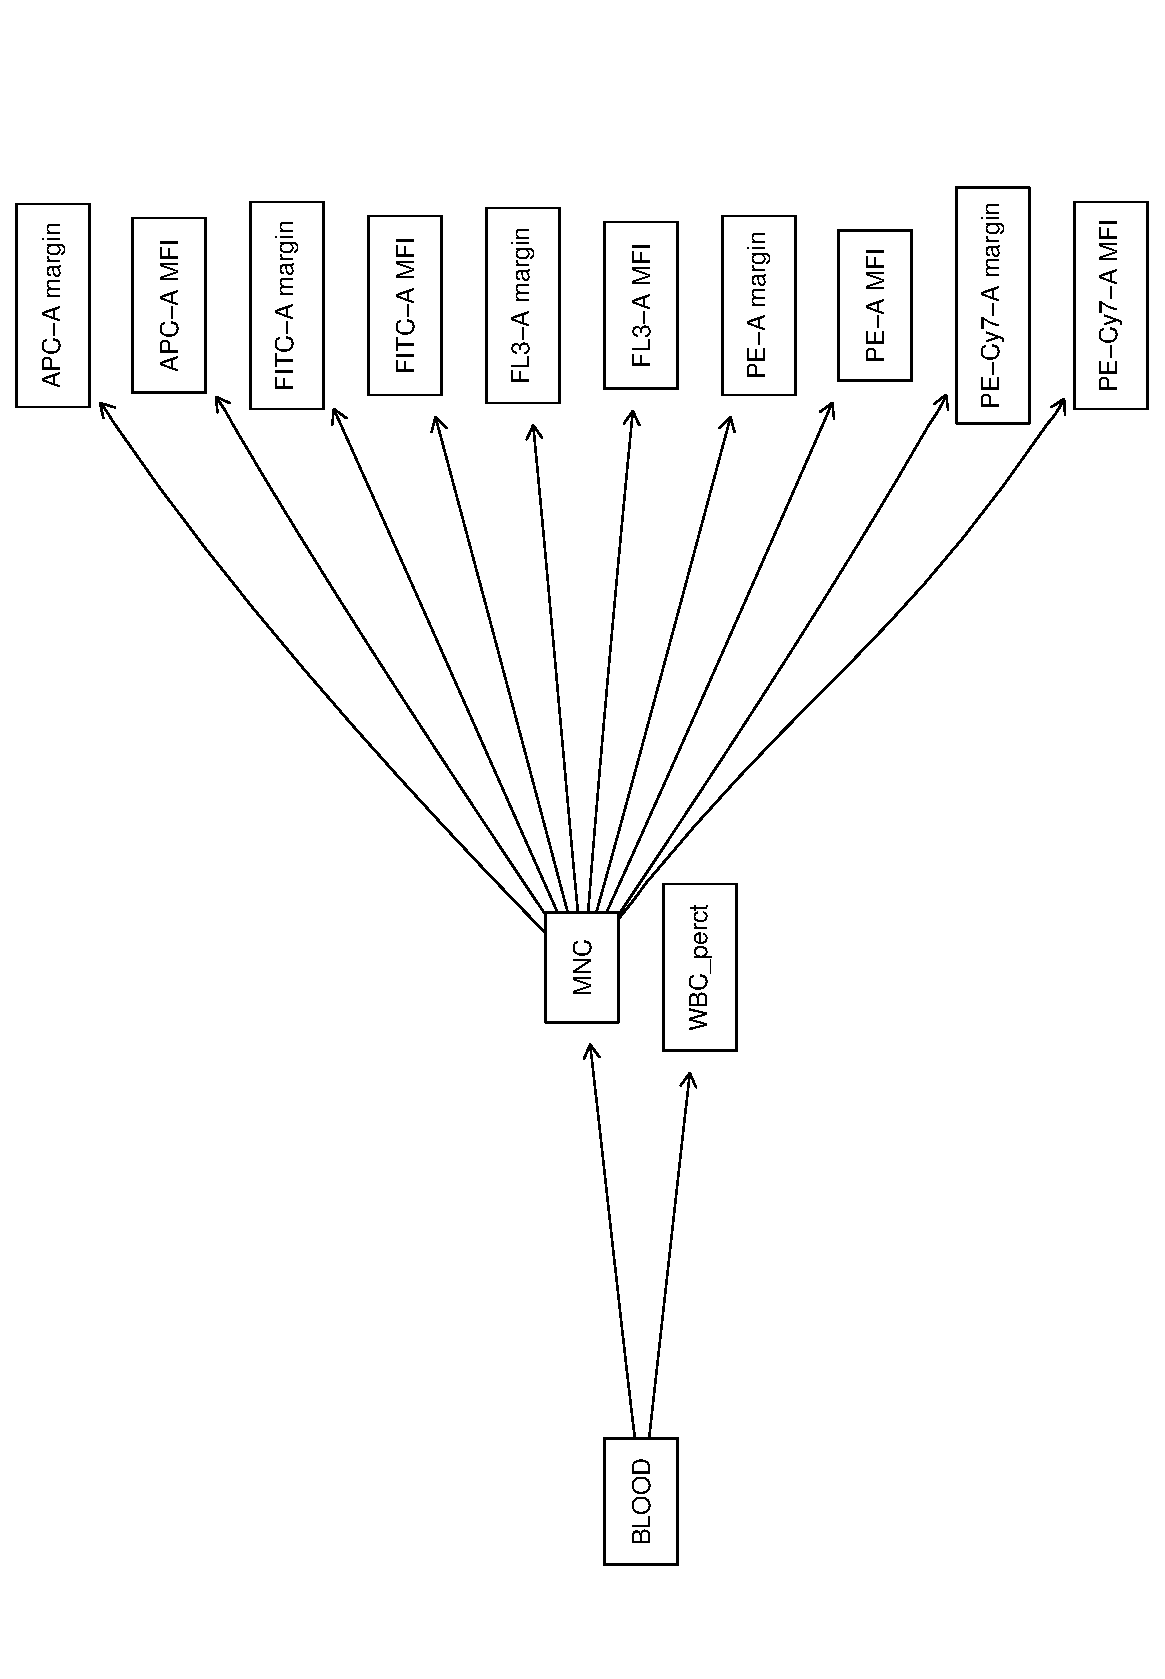
\includegraphics[totalheight=120mm,angle=-90]{image/gatingHierarchy.pdf}
\caption{gating template} 
\end{figure}

\subsection{Extracting the statistics}
The second step is to use function texttt{getQAStats} to extract statistics from
the gating hierarchies of \texttt{GatingSet} and re-organize them in a database that is more suitable
for query and grouping. Further quality assessment will be performed
based on this database with different filters and at different conditioning
levels.

\begin{verbatim}
getQAStats(db)
\end{verbatim}

\subsection{Defining qaTasks} 
One important step before the actual outlier detection is to tell the algorithm:
1.the cell population of interest;
2.type of statistics to use;
3.the sample group within which the statistics is monitored.
 
We use \texttt{qaTask} class as a general container that allow users to
define different QA tasks. The class stores the cell population information
in \texttt{pop} slot and uses \texttt{formula} object as a
compact and generic symbolic form to define the statistical property and sample
groups that are involved. It is generally of the form $y \sim x|g1*g2*...$ ,
y is the statistical property to be checked, it is one of the four types:
				
				"MFI": 
					Median Fluorescence Intensity of the cell population specified by \texttt{qaTask},
			
				"percent": 
						the percentage of the cell population specified by \texttt{qaTask} in the parent population, 
			
				"count": 
						the number of events of the cell population specified by \texttt{qaTask},
			
				"spike": 
						the variance of intensity over time of each channel ,which indicating the stability of the fluorescence intensity.

x specifies the variable plotted on x-axis (such as date) in \texttt{plot} method.

g1,g2,.... are the conditioning variables, which divide the data into subgroups. 
The outlier detection is conducted whitin each individual group. 
They may be omitted,which indicates that the outliers detection is peformed
in the entire sample set.

We provide a convenient function \texttt{makeQaTask} to read these task
definition from a spreadsheet and construct multiple \texttt{qaTask} objects at
once. Each entry in the spreadsheet corresponds to one QA task and contains these essential
information in different columns. Users can
also create the individual \texttt{qaTask} directly by using \texttt{new} method.

\begin{verbatim}
qaTask.list<-makeQaTask(db,checkListFile)
\end{verbatim}


\subsection{Quality assessment and visualiztion} 
\texttt{qaCheck} and \texttt{plot} perform the actual quality assessment and
visualization based on the definitions stored in \texttt{qaTask} object. For example, RBC
Lysis efficiency is measured by the percentage of the white blood cell(WBC) population and its \texttt{qaTask} is defined as:
\begin{verbatim}
>qaTask.list[["RBCLysis"]]
qaTask: RBCLysis 
Level : Tube 
Description : Sufficient RBC lysis 
Plot type:  xyplot
Gated node:  WBC_perct
Default formula :percent ~ RecdDt | Tube
\end{verbatim}
According to the formula \emph{percent$\sim$RecordDate$|$Tube}, the statistical
property \emph{percent} will be used for the cell population \emph{WBC} and the
data will be grouped by \emph{Tube}(or staining panel). The \emph{percent}
will be plotted against \emph{RecordDate} in a dotplot.Here is how the QA is
conducted:
\begin{verbatim}
qaCheck(qaTask.list[["RBCLysis"]],outlierfunc=outlier.cutoff,lBound=0.8)
\end{verbatim}
\texttt{qaCheck} method reads the statistics of interest from the database
and detect the outliers within each sample group. The
\texttt{outlierfunc} can be any outlier function as long as takes a numeric
vector as input and returns a logical vector as the output. 
Here the function \emph{outlier.cutoff} provided by the package is used.
\emph{lBound} is the threshold equivalent to $\leq$ (\emph{uBound} for $\geq$).
By default \texttt{plot} method plots all the data specifiled by \texttt{qaTask}.
A filter can be passed through argument \emph{subset} to select a small subset to
visualize.
 \begin{verbatim}
plot(qaTask.list[["RBCLysis"]],subset="Tube=='CD8/CD25/CD4/CD3/CD62L'")
\end{verbatim}%TODO:merge two plots into one figure here
\begin{figure}[h]
\begin{tabular}{cc}
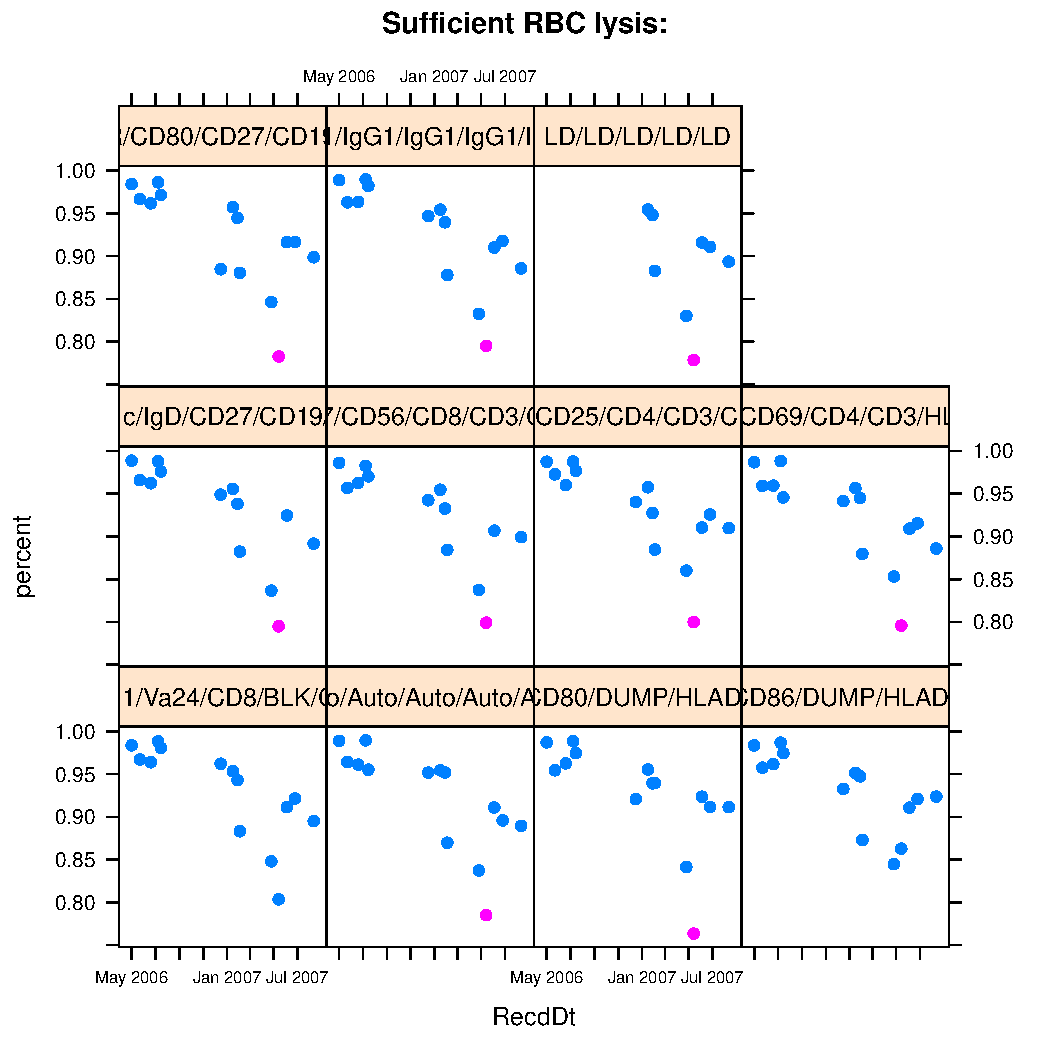
\includegraphics[width=0.5\textwidth]{image/RBCLysis_all.pdf}&
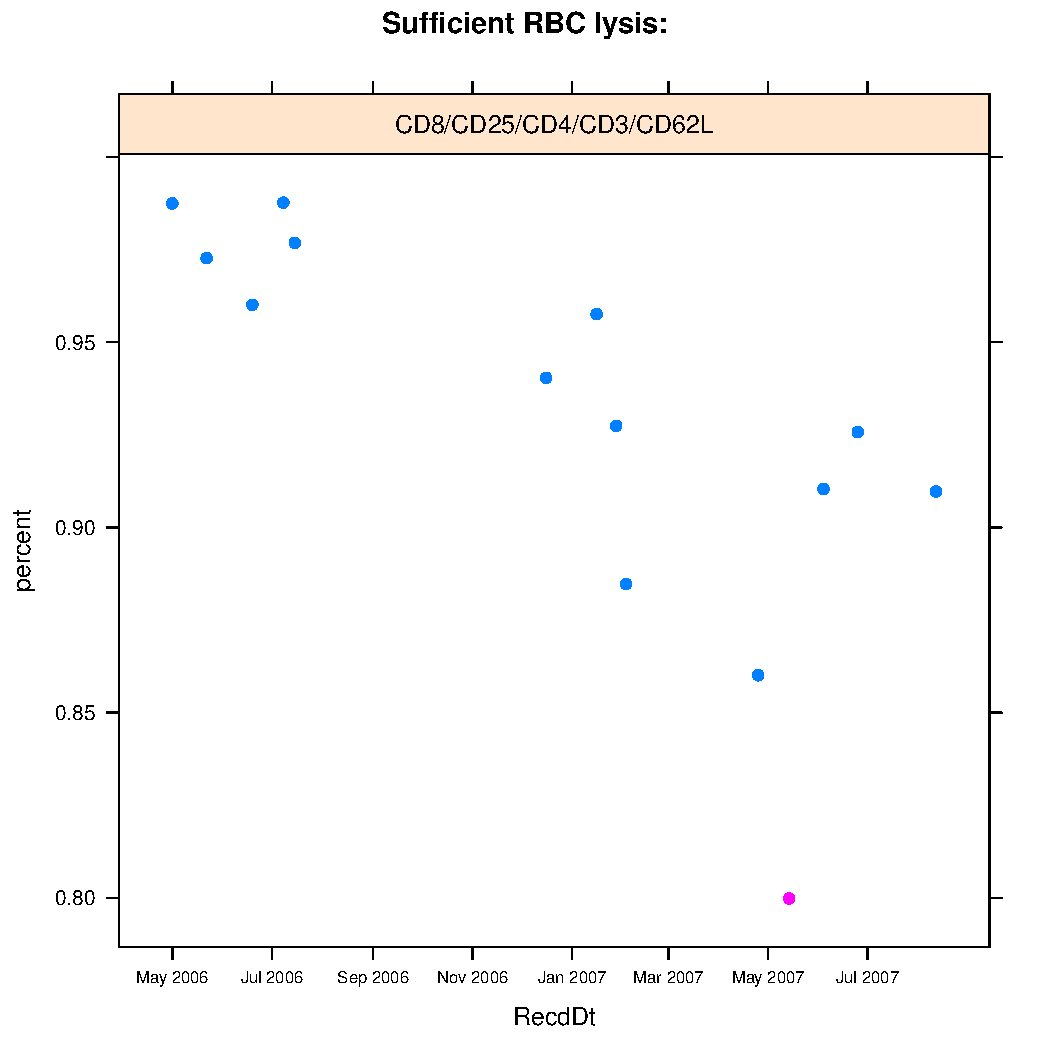
\includegraphics[width=0.5\textwidth]{image/RBCLysis.pdf}
\end{tabular}
\caption{QA result of RBC lysis efficiency} 
\end{figure}
\clearpage
$x$ term in the formula is normally used for plotting. When $plotType$
of the \texttt{qaTask} is defined as "bwplot" (boxplot),$x$ is also considered as a conditioning variable that divides the data into subgroups within which the \texttt{outlierfunc} is applied. For
example:
\begin{verbatim}
>qaTask.list[["MNC"]]
qaTask: MNC 
Level : Assay 
Description : Consistency of Lymphocyte/MNC Gate 
Plot type:  bwplot
Gated node:  MNC
Default formula :percent ~ coresampleid
\end{verbatim}
This qaTask detects the significant variance of MNC cell populations among
aliquots that have the same \emph{coresampleid}. Plot type of this object tells the method to group data by "coresampleid".
\begin{verbatim}
qaCheck(qaTask.list[["MNC"]],outlierfunc=qoutlier,alpha=1.5)
\end{verbatim}
Interquartile Range based outlier detection function is used here.The boxplot is
plotted by:
\begin{verbatim}
plot(qaTask.list[["MNC"]])
\end{verbatim}
%\begin{figure}[h]
%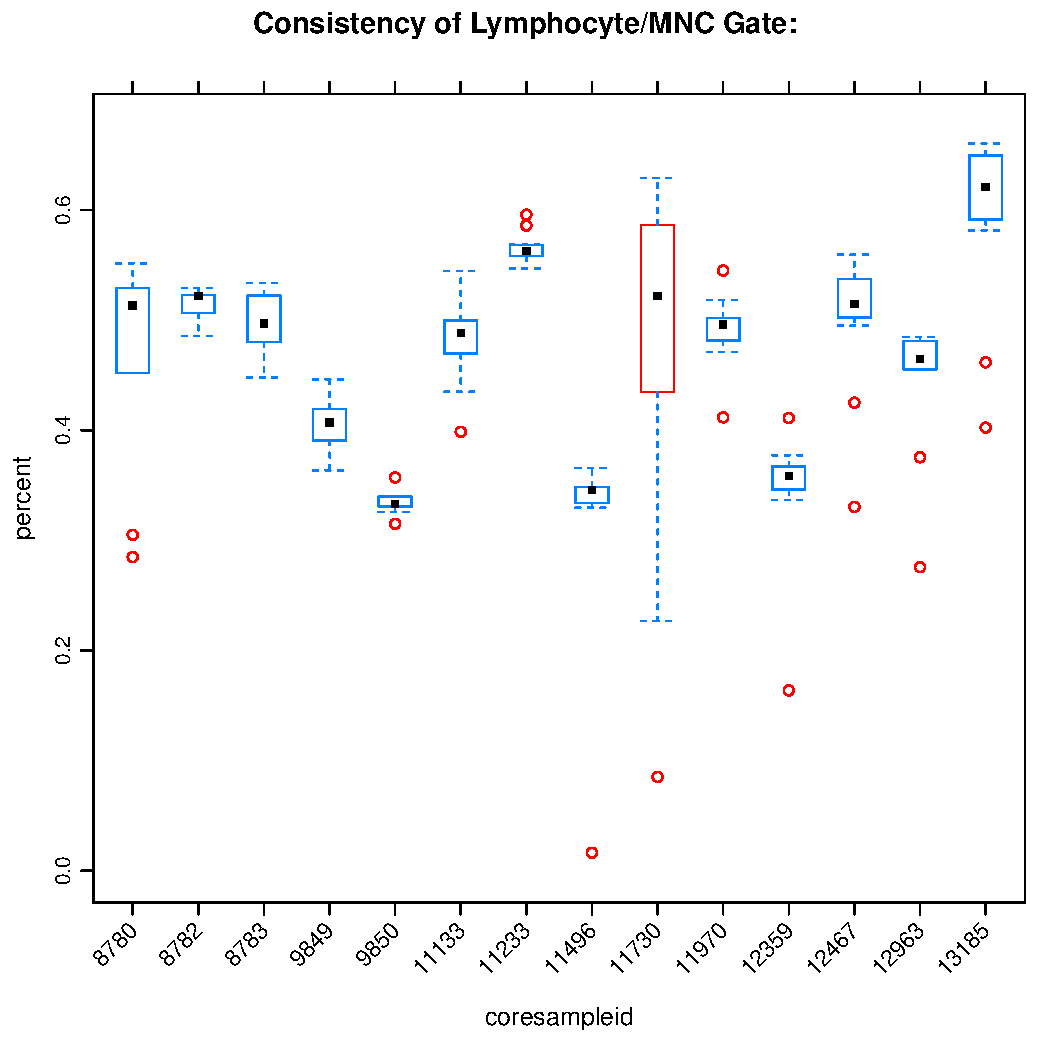
\includegraphics[width=120mm,height=80mm]{image/MNC.pdf}
%\caption{QA result of MNC consistency} 
%\end{figure}
\begin{figure}[h]
\begin{tabular}{cc}
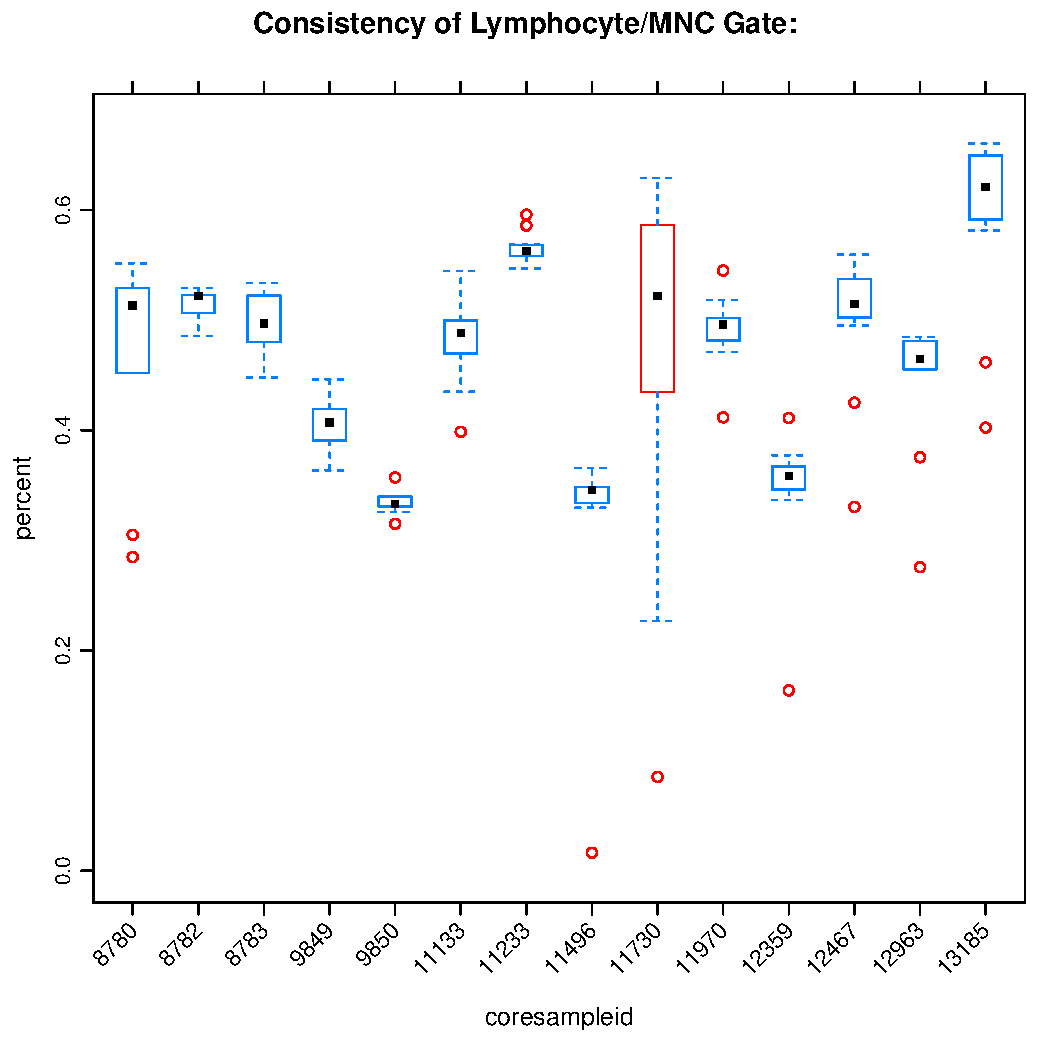
\includegraphics[width=0.5\textwidth]{image/MNC.pdf}&
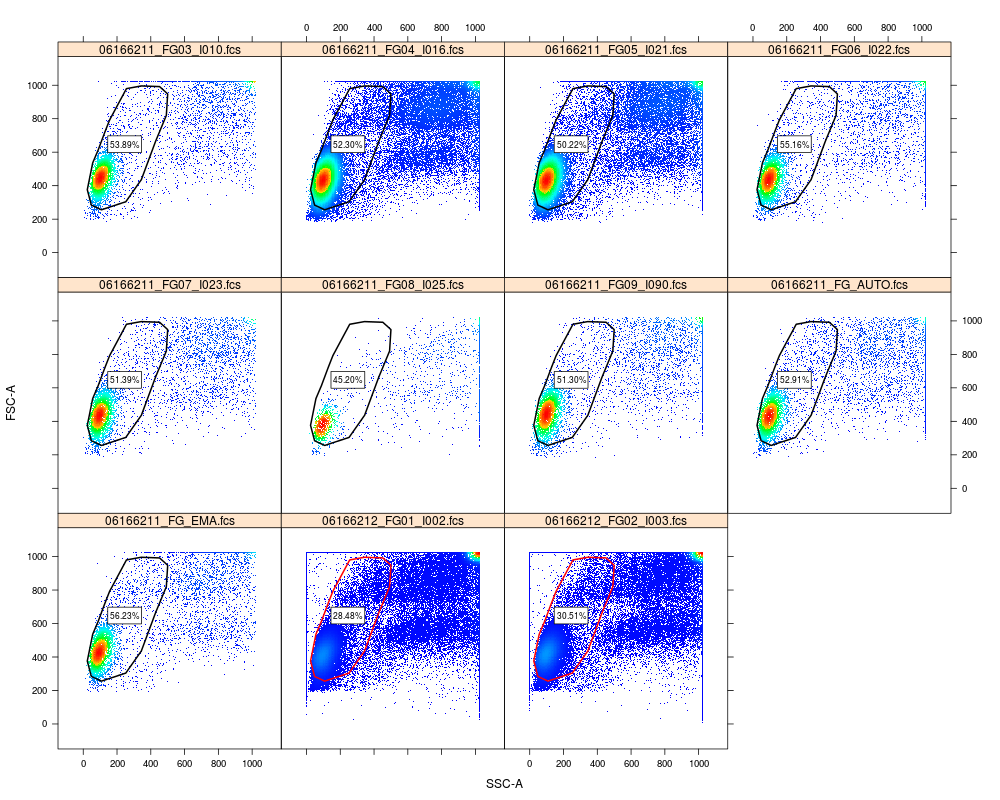
\includegraphics[width=0.5\textwidth]{image/s_8780_MNC_proportion.png}
%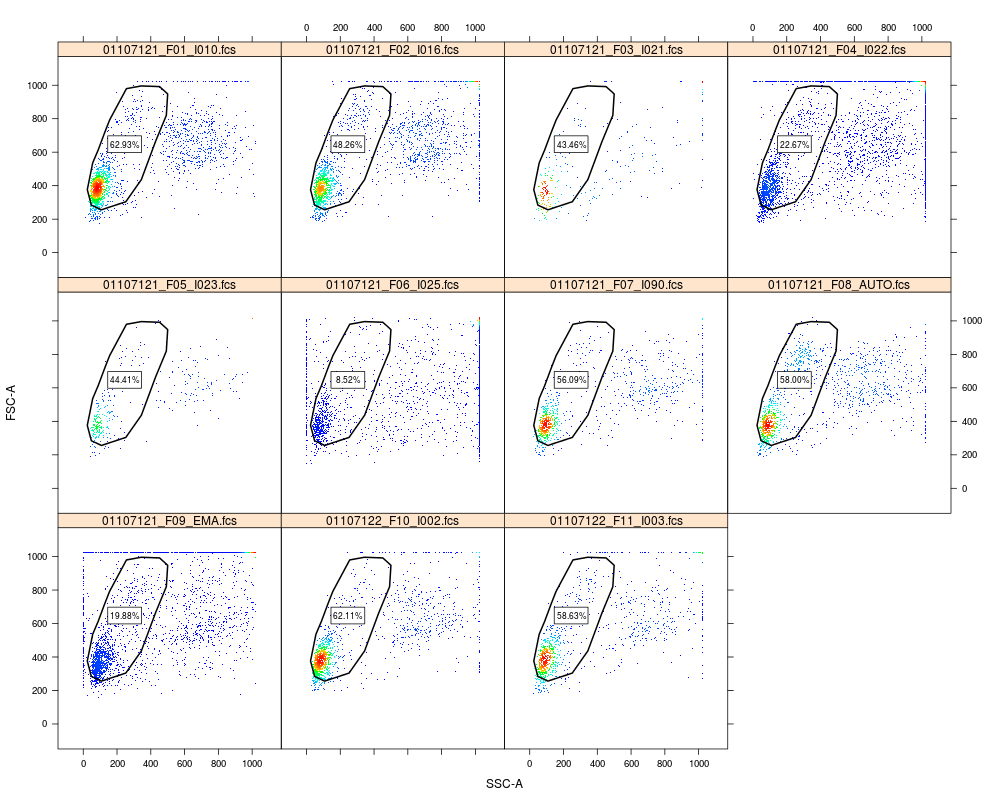
\includegraphics[width=0.5\textwidth]{image/s_11730_MNC_proportion.png}
\end{tabular}
\caption{scatterplots of MNC gate} 
\end{figure}
The red circles in the boxplot indicate the possible outlier samples and the box
flagged with red color indicates the entire sample groups have significant
variances and require the further investigation.Optionally,\texttt{plot} method
provides the plots in svg format displaying the
details of individual sample as tooltips and containing hyperlinks to the
2D scatterplots for the individual FCS files.
			
The \texttt{formula} can be modified through the argument of \texttt{qaCheck}
and \texttt{plot} methods allowing users to interactively explore the data by
changing different conditioning levels and applying simple aggregations to the
statisics. The formula defined by the QA task below extracts the
"percent" independently for each individual channel:
\begin{verbatim}
>qaTask.list[["BoundaryEvents"]]
qaTask: BoundaryEvents 
Level : Channel 
Description : Off-scale Boundary Events 
Plot type:  xyplot
Gated node:  margin
Default formula :percent ~ RecdDt | channel
\end{verbatim}
IF we want to combine boundary events of all channels and
check the overall percentage for each fcs file, the aggregation function "sum"
can be simply added to the formula as well as the conditioning variable changed
to \emph{fcsFile} indicating that data is grouped at FCS file level.
\begin{verbatim}
qaCheck(qaTask.list[["BoundaryEvents"]]
		,sum(percent) ~ RecdDt | fcsFile
		,outlierfunc=outlier.cutoff
		,uBound=0.0003
		)
\end{verbatim}
The QA results will still be visualized in chanel-wise pannels by using the
original formula:
\begin{verbatim}		
plot(qaTask.list[["BoundaryEvents"]],percent ~ RecdDt | channel)
\end{verbatim}
\begin{figure}[h]
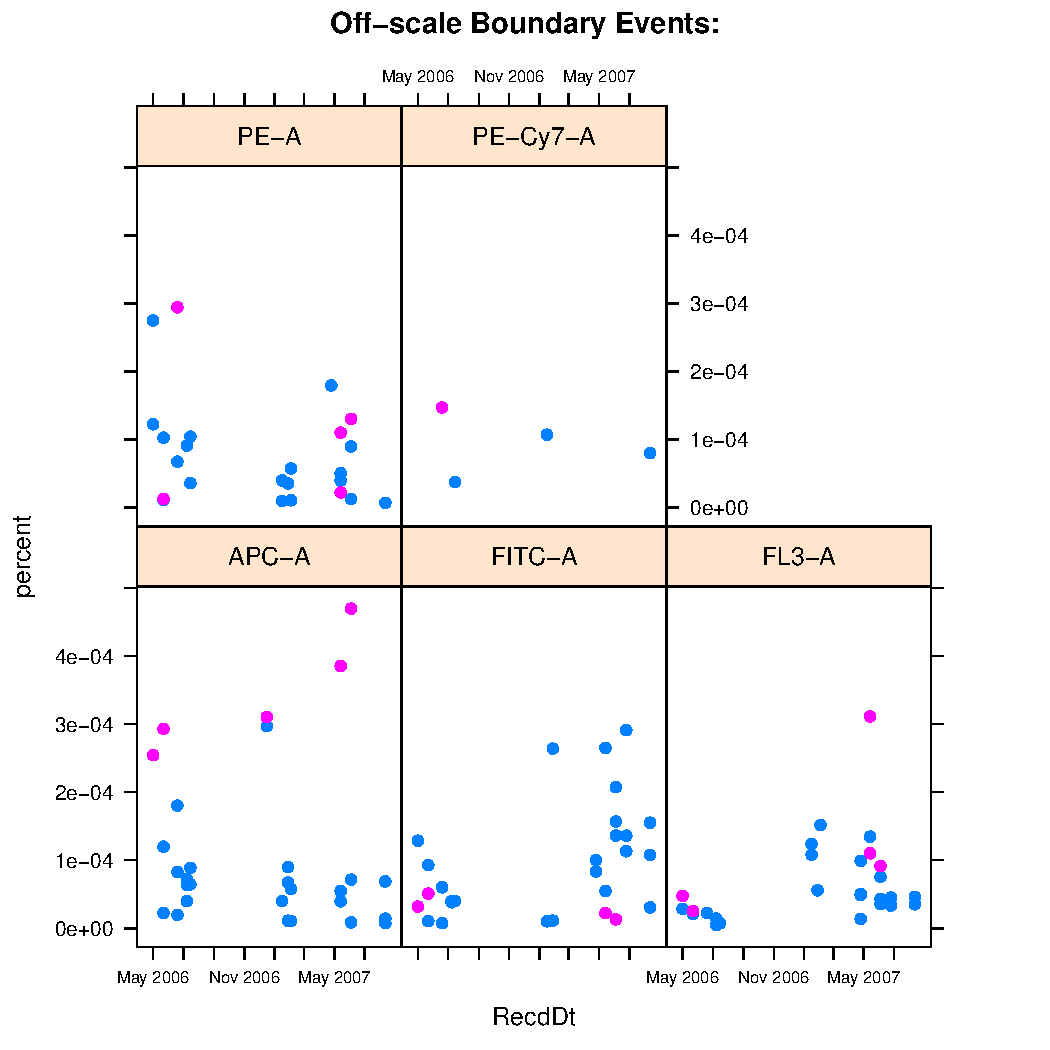
\includegraphics[totalheight=120mm]{image/BoundaryEvents.pdf}
\caption{QA result of of boundary events} 
\end{figure}
\clearpage
With all the statistical data accumulated in the QA database overtime, it is
easy to perform QA tasks over a long period of the time for longitudinal
studies. Below is the QA for monintoring fluorescence stability overtime using
t-distribution based outlier detection function.
\begin{verbatim}
qaCheck(qaTask.list[["MFIOverTime"]]
		,outlierfunc=outlier.t
		,rFunc=lm
		,alpha=0.05
		)
plot(qaTask.list[["MFIOverTime"]],y=MFI~RecdDt|stain
		,subset="channel%in%c('FITC-A')"
		,rFunc=lm
	)
\end{verbatim}
Note that the linear regression is applied in each group in order to capture the significant MFI change over time.
The sample outliers within each group is also detected based on the residue.
\begin{figure}[h]
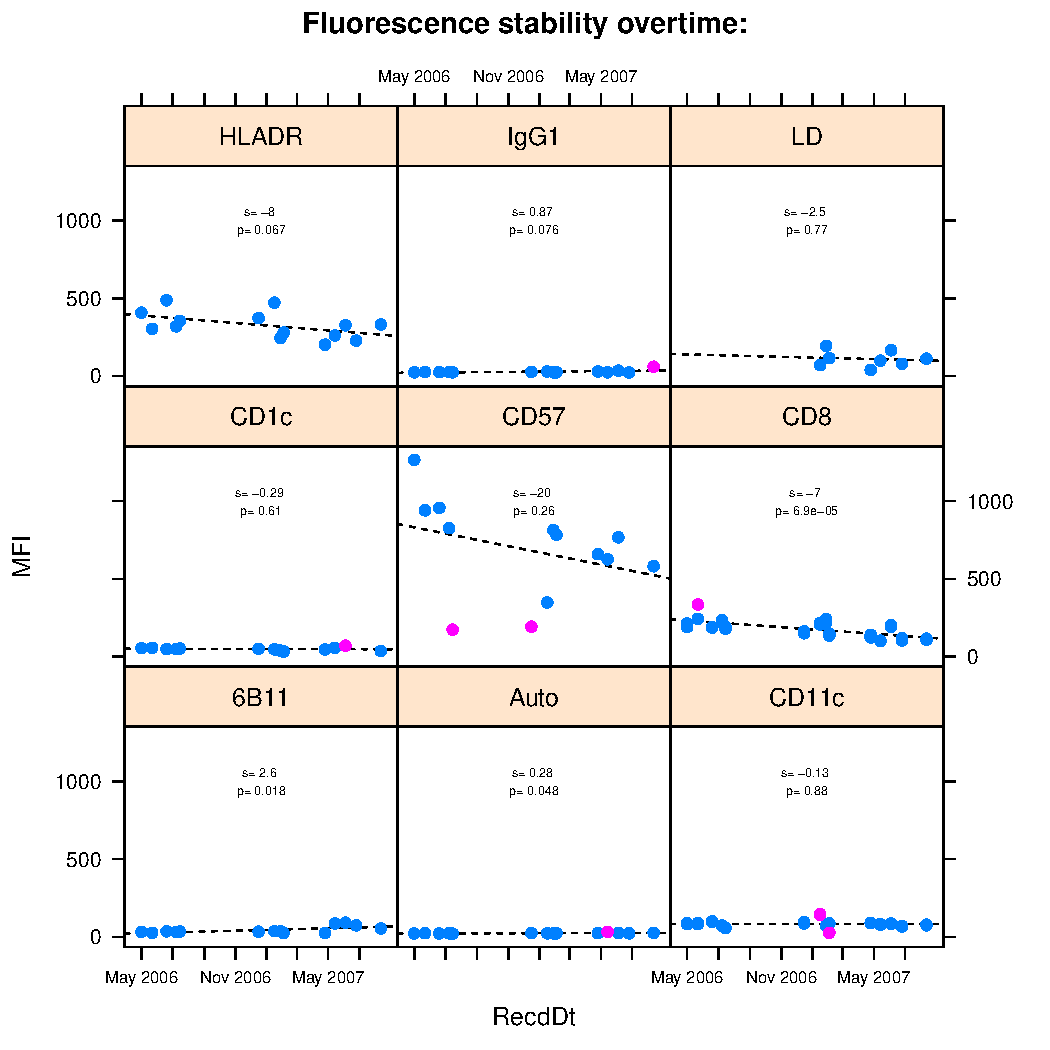
\includegraphics[height=100mm]{image/MFI.pdf}
\caption{QA result of of MFI stability} 
\end{figure}
\clearpage
\subsection{Creating quality assessment report}
Besides the visualization of each QA
task using the \texttt{plot} method,we provide \texttt{qa.report} function
to create QA report in HTML format for all QA tasks.The report contains the
summary tables and SVG plots.

\section*{Conclusion}
\textbf{QUAliFiER} is a recently developed \textbf{R} package dedicated to
quality assessment of gated FCM data, addressing the increasing demand for
software capable of processing and minitor the voluminous amount of FCM data
efficiently via an objective, reproducible and automated means. 
 It calculates and stores the statiscis from the gated FCM data and conduct
 QA checks and visualization interactively.

  
%%%%%%%%%%%%%%%%%%%%%%%%%%%%%%%%
\section*{Availability and requirements}
Project name: QUAliFiER\pb
Project homepage: \url{http://bioconductor.org}\pb
Operating systems: Platform independent\pb
Programming language: R\pb
Other requirements: R, Bioconductor\pb
License: Artistic 2.0\pb

\bigskip

%%%%%%%%%%%%%%%%%%%%%%%%%%%%%%%%
\section*{Author's contributions}
    WJ,GF and RG developed the methodology and software, and performed the
    analyses. AS participated in its design and coordination.  WJ and GF draft
    the manuscript.  All authors read and approved the final manuscript.

    

%%%%%%%%%%%%%%%%%%%%%%%%%%%
\section*{Acknowledgements}
  \ifthenelse{\boolean{publ}}{\small}{}
  The authors thank  xxx for their advice on xxx. This work was supported by the
  NIH grant xxx from xxx.
 
%%%%%%%%%%%%%%%%%%%%%%%%%%%%%%%%%%%%%%%%%%%%%%%%%%%%%%%%%%%%%
%%                  The Bibliography                       %%
%%                                                         %%              
%%  Bmc_article.bst  will be used to                       %%
%%  create a .BBL file for submission, which includes      %%
%%  XML structured for BMC.                                %%
%%  After submission of the .TEX file,                     %%
%%  you will be prompted to submit your .BBL file.         %%
%%                                                         %%
%%                                                         %%
%%  Note that the displayed Bibliography will not          %% 
%%  necessarily be rendered by Latex exactly as specified  %%
%%  in the online Instructions for Authors.                %% 
%%                                                         %%
%%%%%%%%%%%%%%%%%%%%%%%%%%%%%%%%%%%%%%%%%%%%%%%%%%%%%%%%%%%%%

\newpage
{\ifthenelse{\boolean{publ}}{\footnotesize}{\small}
 \bibliographystyle{bmc_article}  % Style BST file
  \bibliography{cytometry} }     % Bibliography file (usually '*.bib' ) 

%%%%%%%%%%%

\ifthenelse{\boolean{publ}}{\end{multicols}}{}

%%%%%%%%%%%%%%%%%%%%%%%%%%%%%%%%%%%
%%                               %%
%% Figures                       %%
%%                               %%
%% NB: this is for captions and  %%
%% Titles. All graphics must be  %%
%% submitted separately and NOT  %%
%% included in the Tex document  %%
%%                               %%
%%%%%%%%%%%%%%%%%%%%%%%%%%%%%%%%%%%

%%
%% Do not use \listoffigures as most will included as separate files

\section*{Figures}
  \subsection*{Figure 1 - Sample figure title}
      A short description of the figure content
      should go here.

  \subsection*{Figure 2 - Sample figure title}
      Figure legend text.



%%%%%%%%%%%%%%%%%%%%%%%%%%%%%%%%%%%
%%                               %%
%% Tables                        %%
%%                               %%
%%%%%%%%%%%%%%%%%%%%%%%%%%%%%%%%%%%

%% Use of \listoftables is discouraged.
%%
\section*{Tables}
  \subsection*{Table 1 - Sample table title}
    Here is an example of a \emph{small} table in \LaTeX\ using  
    \verb|\tabular{...}|. This is where the description of the table 
    should go. \par \mbox{}
    \par
    \mbox{
      \begin{tabular}{|c|c|c|}
        \hline \multicolumn{3}{|c|}{My Table}\\ \hline
        A1 & B2  & C3 \\ \hline
        A2 & ... & .. \\ \hline
        A3 & ..  & .  \\ \hline
      \end{tabular}
      }



%%%%%%%%%%%%%%%%%%%%%%%%%%%%%%%%%%%
%%                               %%
%% Additional Files              %%
%%                               %%
%%%%%%%%%%%%%%%%%%%%%%%%%%%%%%%%%%%

\section*{Additional Files}
  \subsection*{Additional file 1 --- Sample additional file title}
    Additional file descriptions text (including details of how to
    view the file, if it is in a non-standard format or the file extension).  This might
    refer to a multi-page table or a figure.

  \subsection*{Additional file 2 --- Sample additional file title}
    Additional file descriptions text.


\end{bmcformat}
\end{document}







